\documentclass[]{article}

\usepackage{mathtools}
\usepackage{listings}
\usepackage{clrscode}
\usepackage{algorithm}
\usepackage{algorithmic}
\usepackage{graphicx}
\usepackage[top=2cm, bottom=2cm, left=2cm, right=2cm]{geometry}
\DeclareMathOperator*{\argmin}{arg\,min}
\DeclareMathOperator*{\argmax}{arg\,max}

\title{Homework 4}
\date{2015-12-1}
\author{Jingwei Zhang 201528013229095}

\begin{document}
    \maketitle
    \section{Problem 1}
    \begin{figure}[H]
        \centering
        %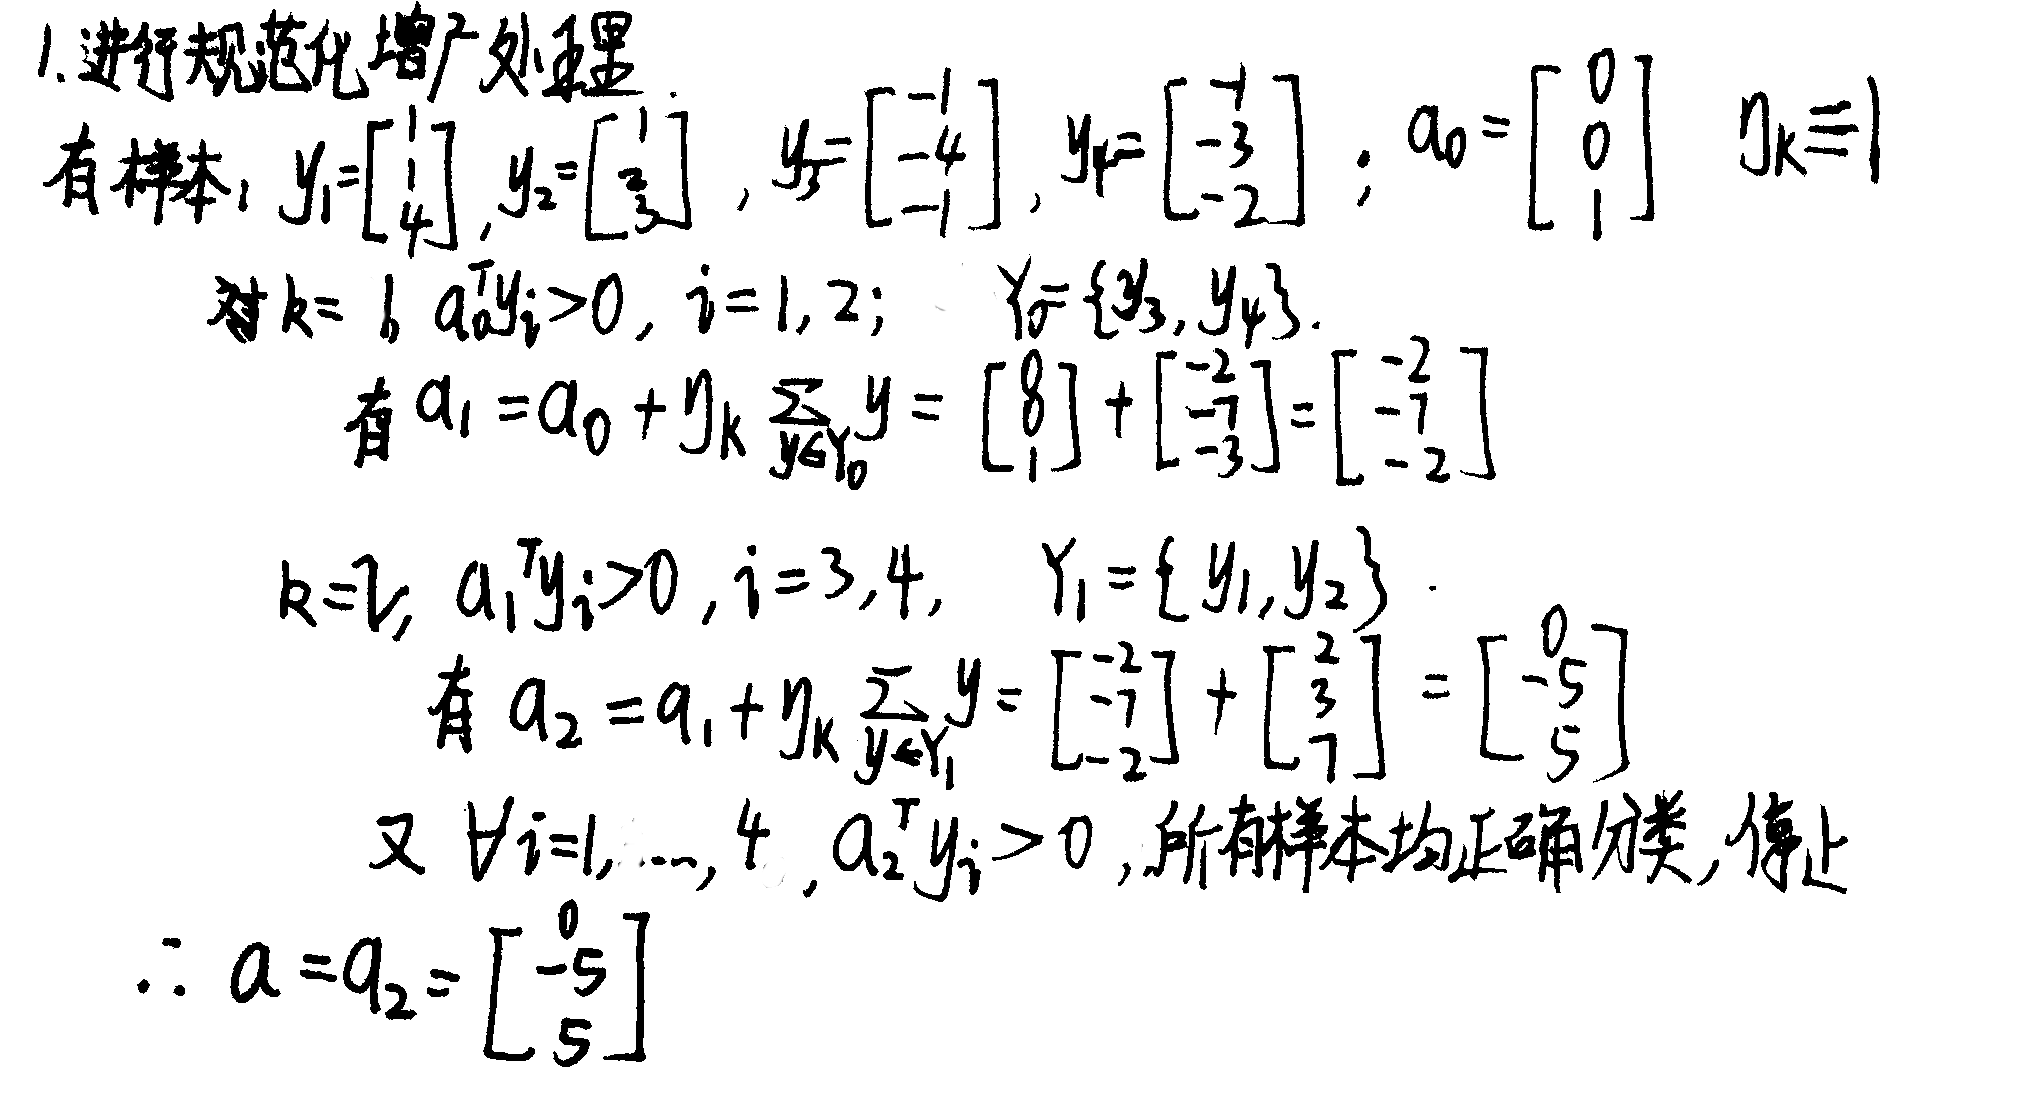
\includegraphics[scale=0.45]{P1.png}
    \end{figure}
    \section{Problem 2}
    \begin{figure}[H]
        \centering
        %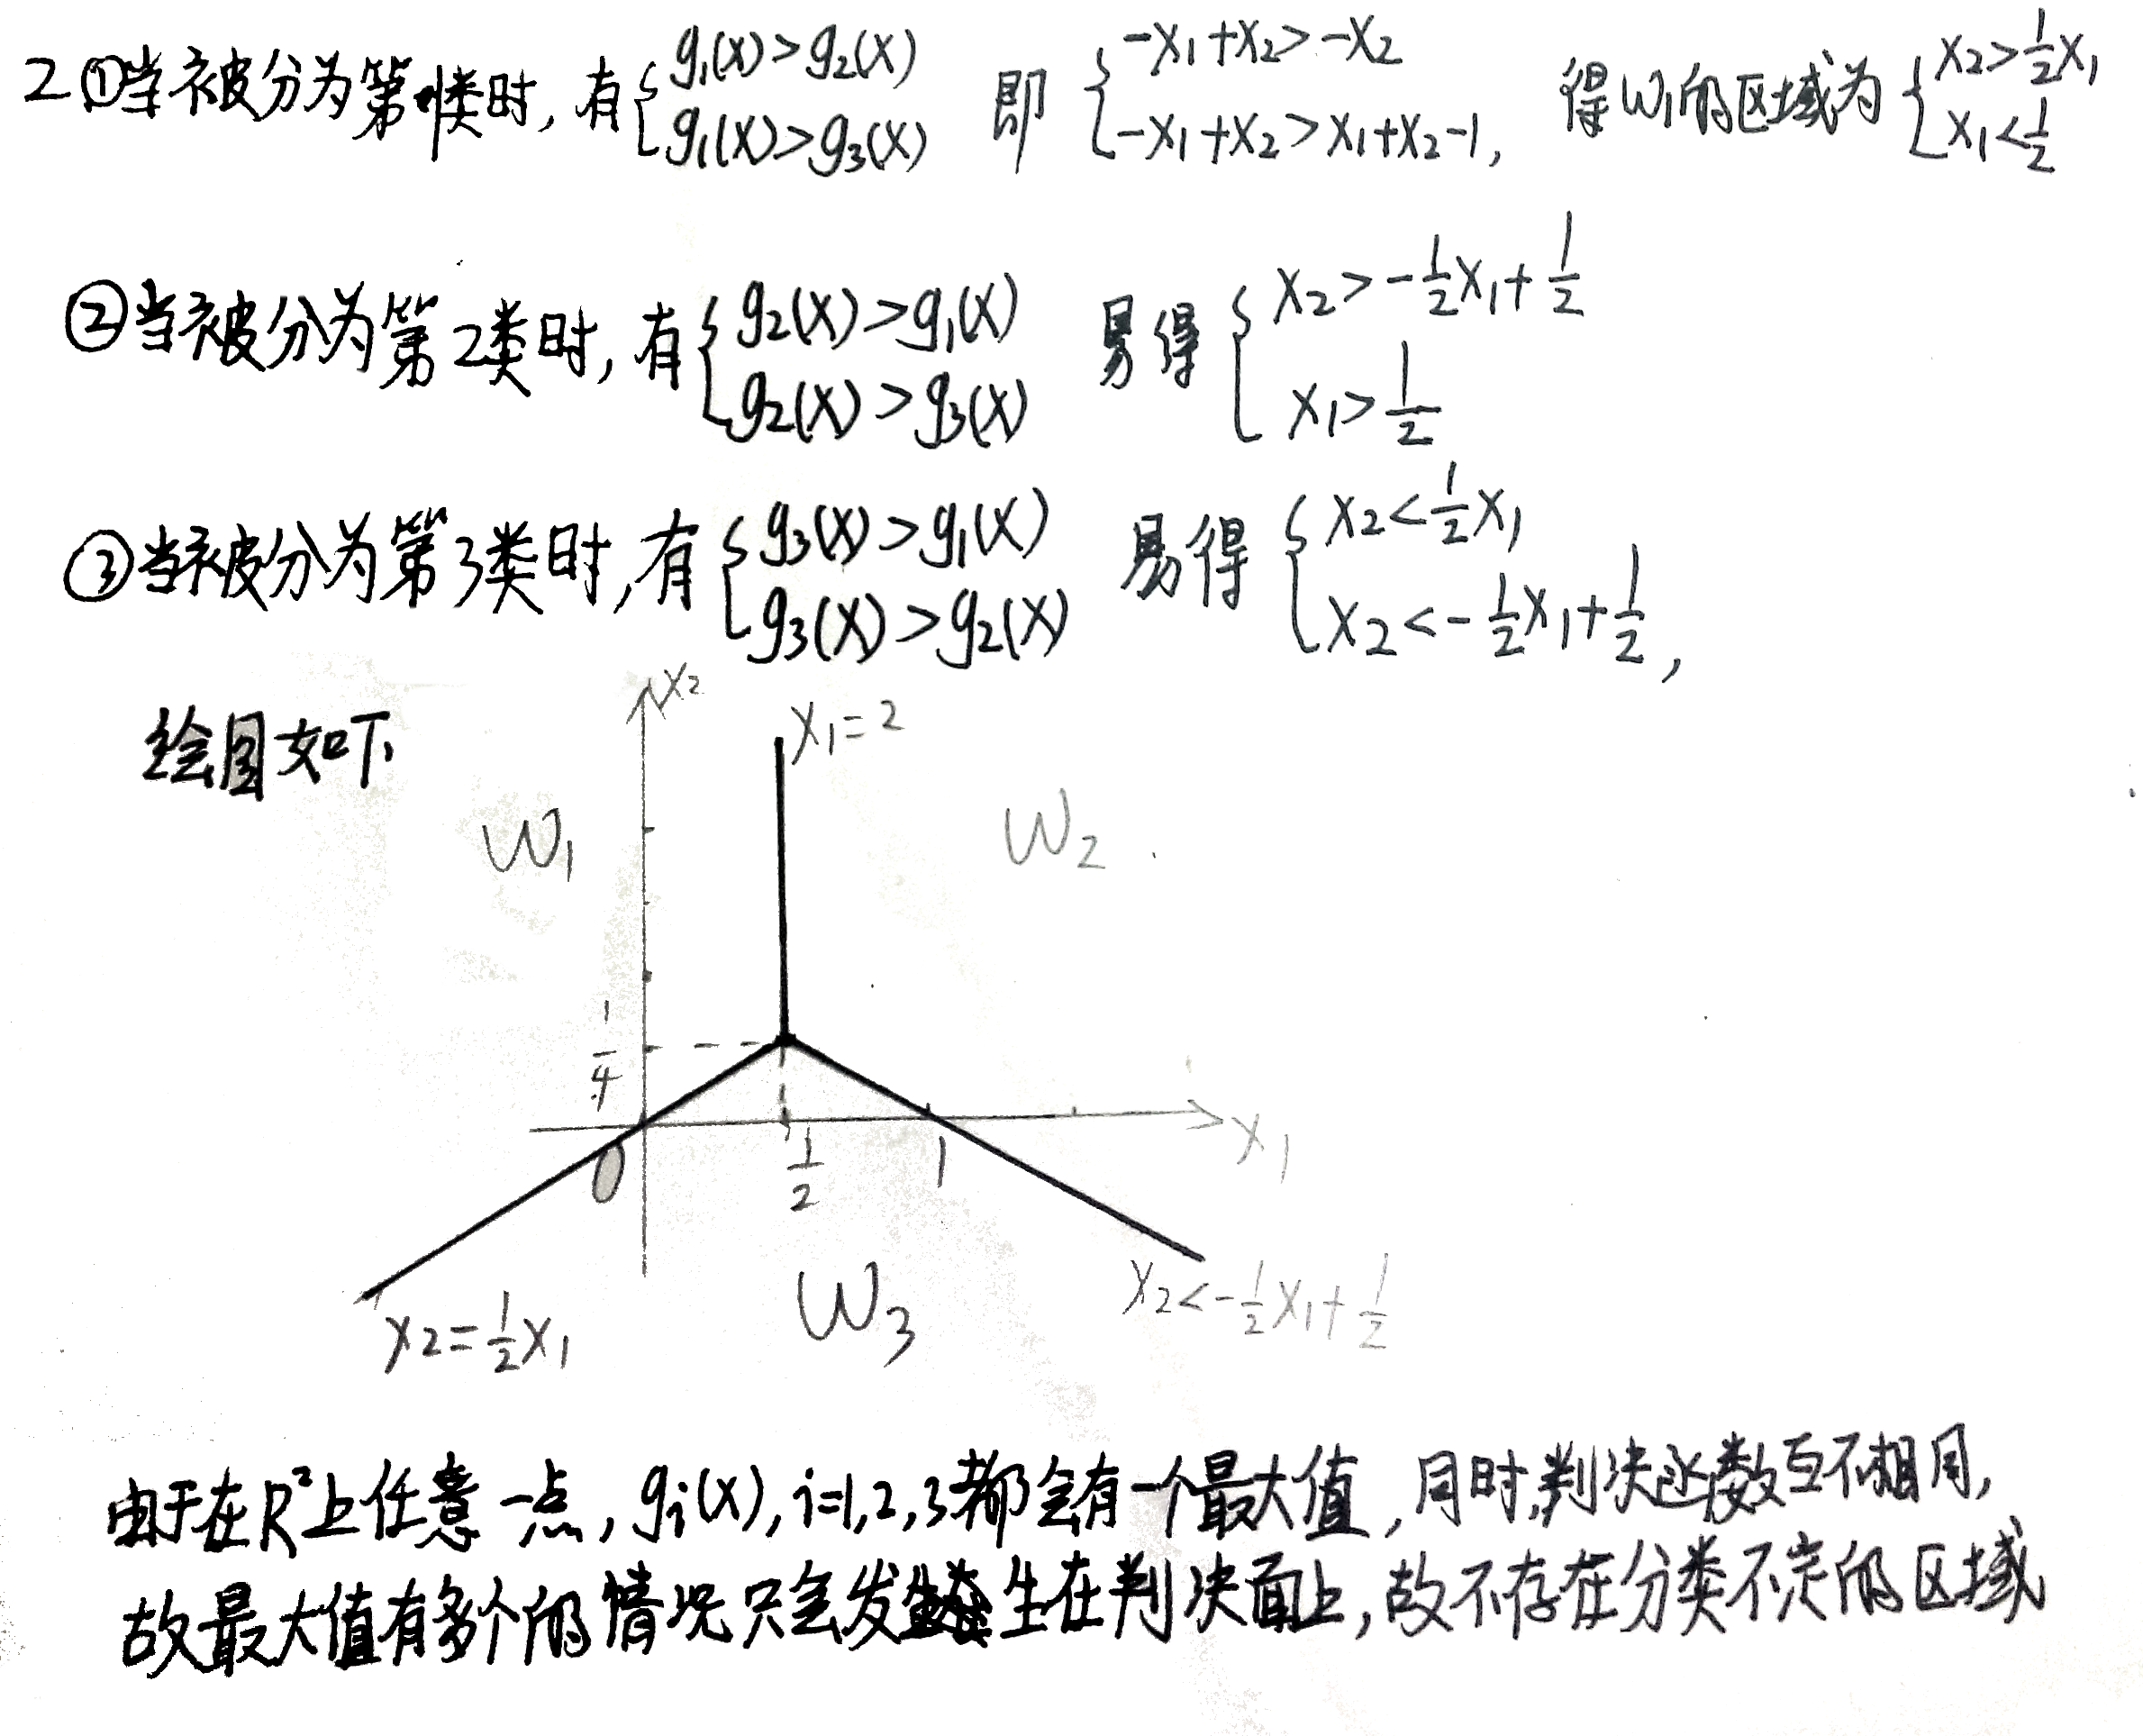
\includegraphics[scale=0.3]{P2.png}
    \end{figure}
    \section{Problem 3}
    \begin{figure}[H]
        \centering
        %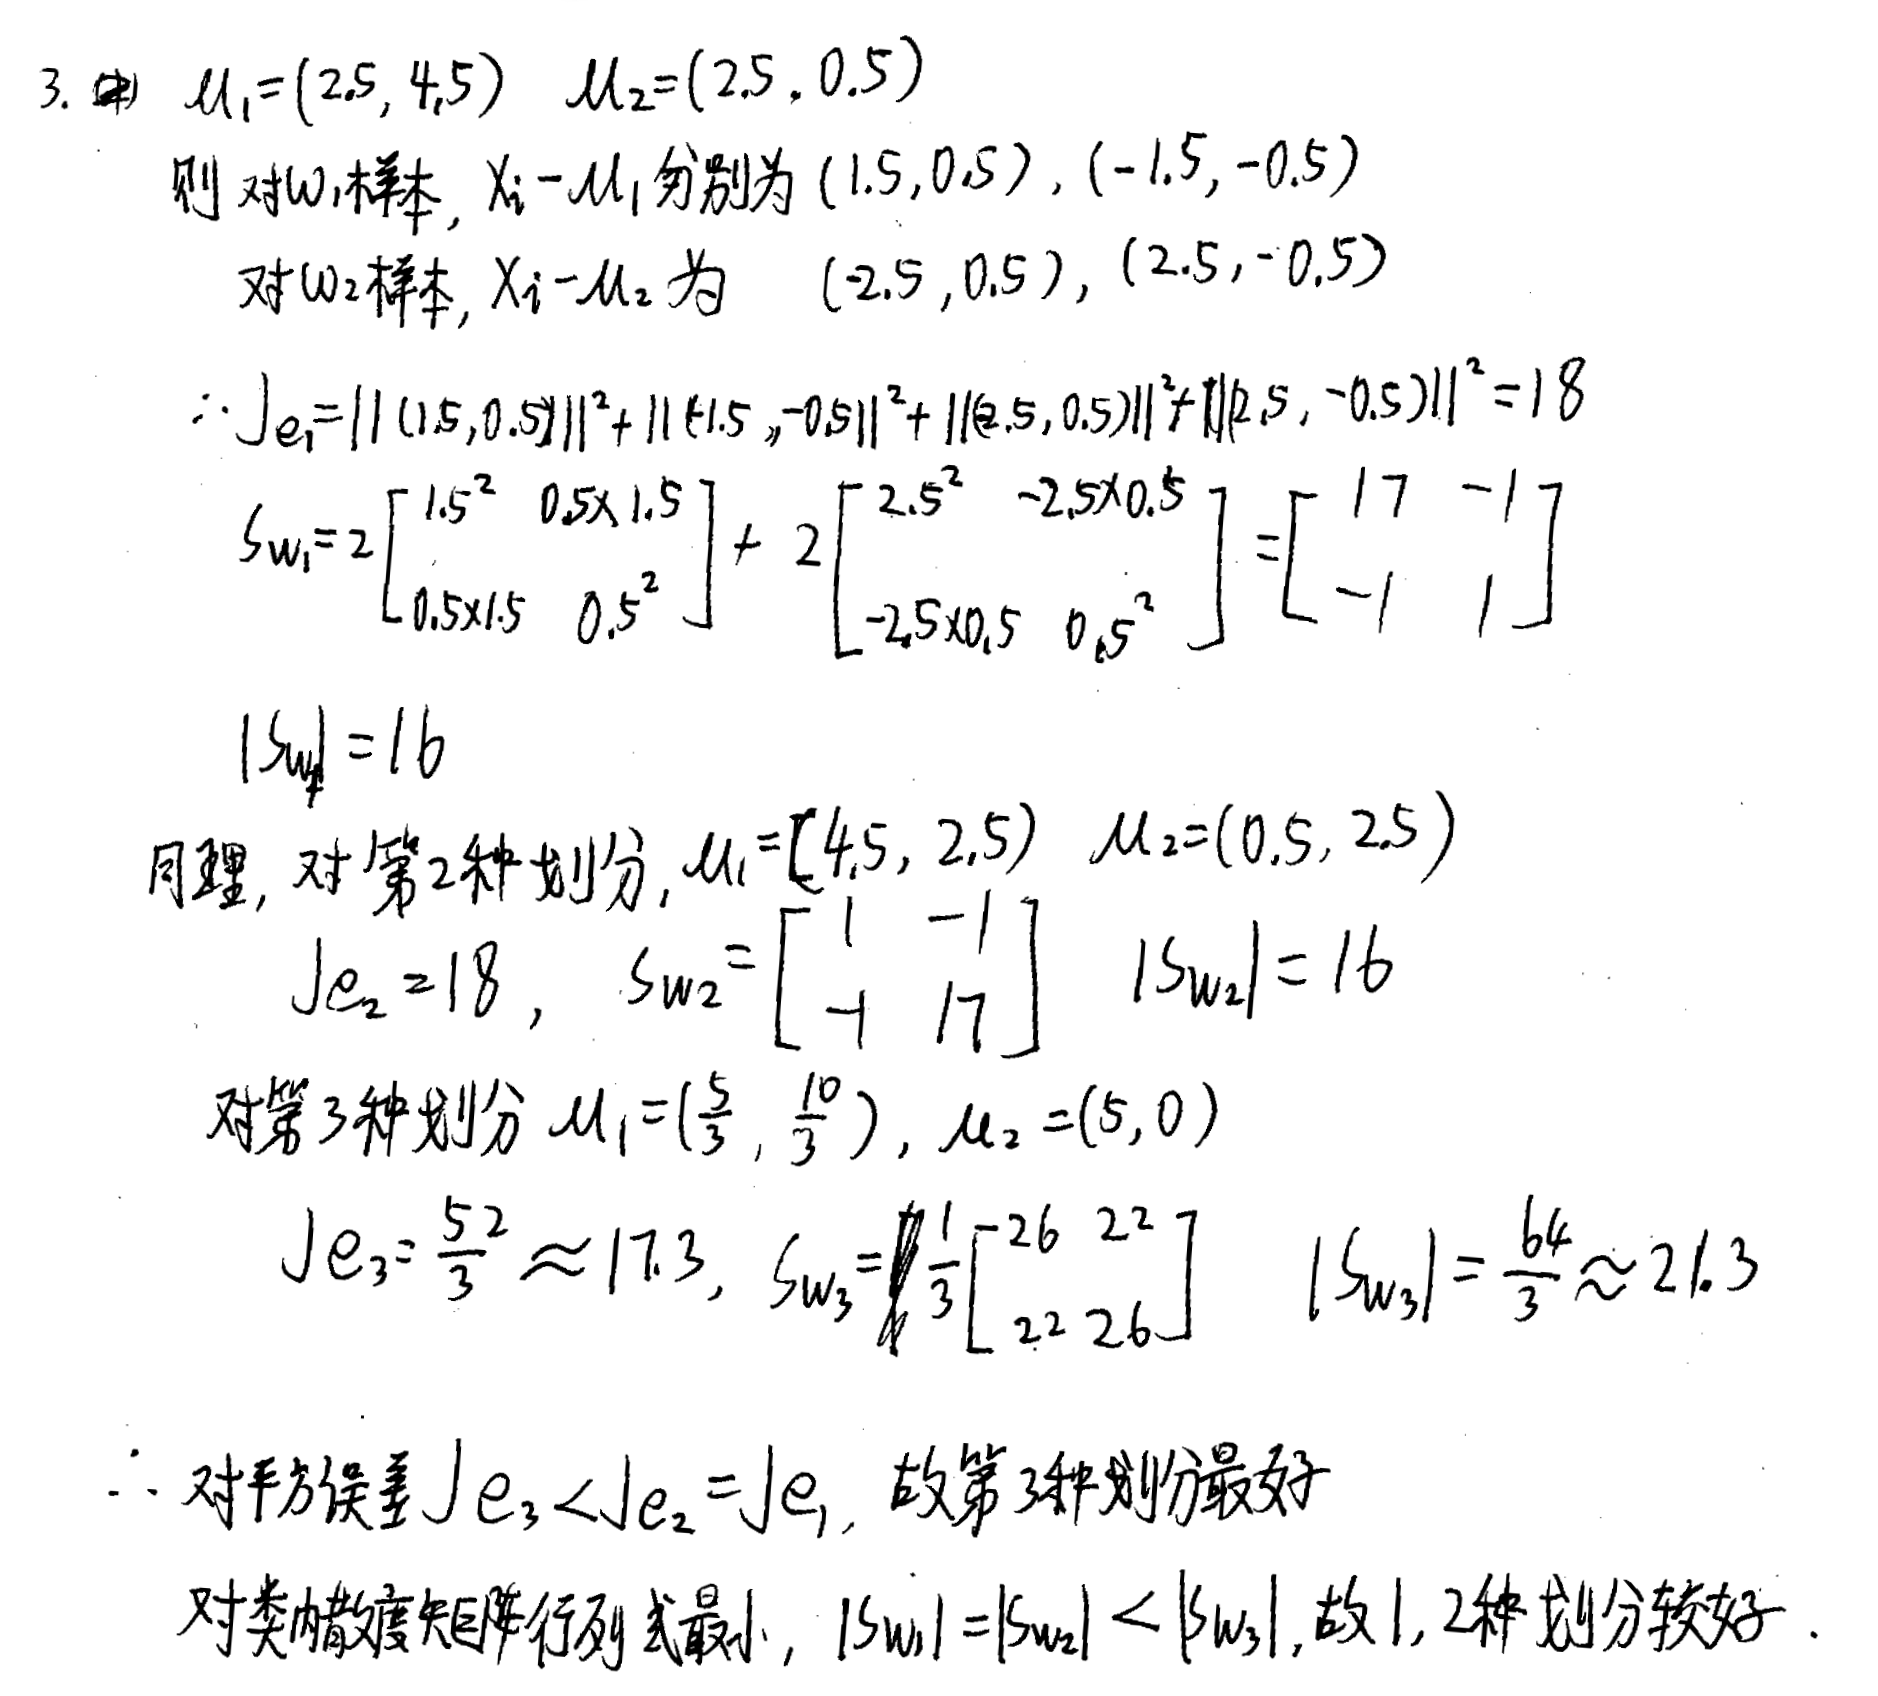
\includegraphics[scale=0.25]{P3.png}
    \end{figure}
    \section{Programming Problem 1}
    \subsection{Result}
    \paragraph{The Number of Iterations:} 23 for $\omega_1$ and $\omega_2$, 16 for $\omega_3$ and $\omega_2$. From figures blow we can find that points of $\omega_3$ and $\omega_2$ are much more scattered, so that $\sum_{y \in Y} y$  will be farther away from current $a$. This will make $a$ converge quicker. 
    \begin{figure}[H]
        \centering
        %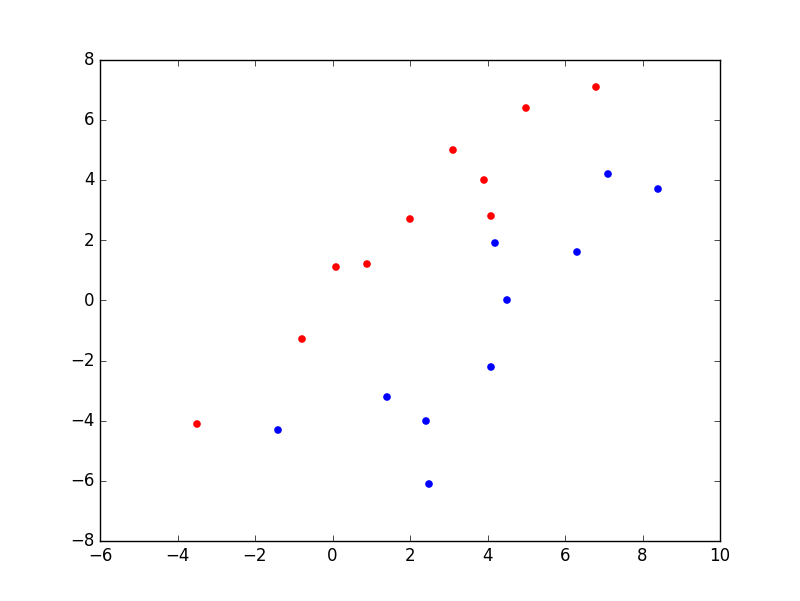
\includegraphics[scale=0.4]{1_1_2.png}
        \caption{Figure for samples belonging to $\omega_1$ and $\omega_2$}
    \end{figure}
    \begin{figure}[H]
        \centering
        %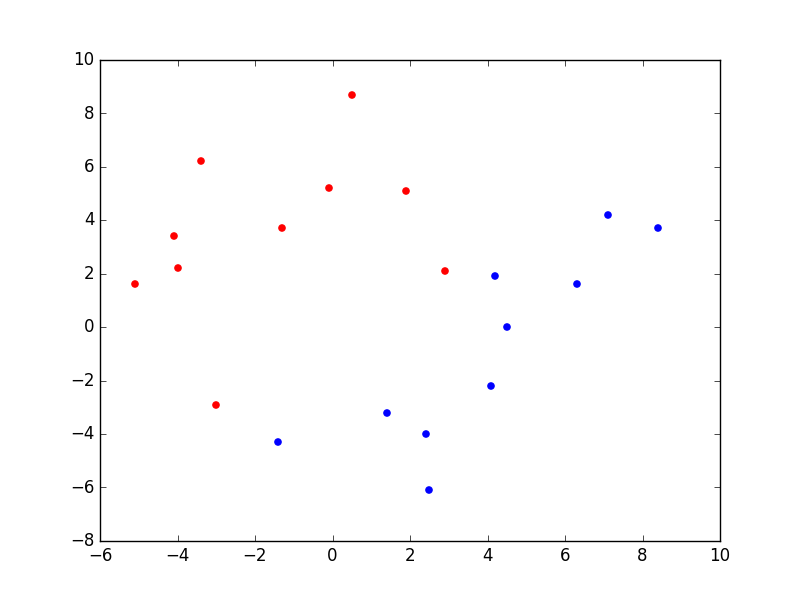
\includegraphics[scale=0.4]{1_3_2.png}
        \caption{Figure for samples belonging to $\omega_3$ and $\omega_2$}
    \end{figure}
    \subsection{Code}
    \lstinputlisting[language=Python]{1.py}


\end{document}